\begin{figure}[h]
    \centering
    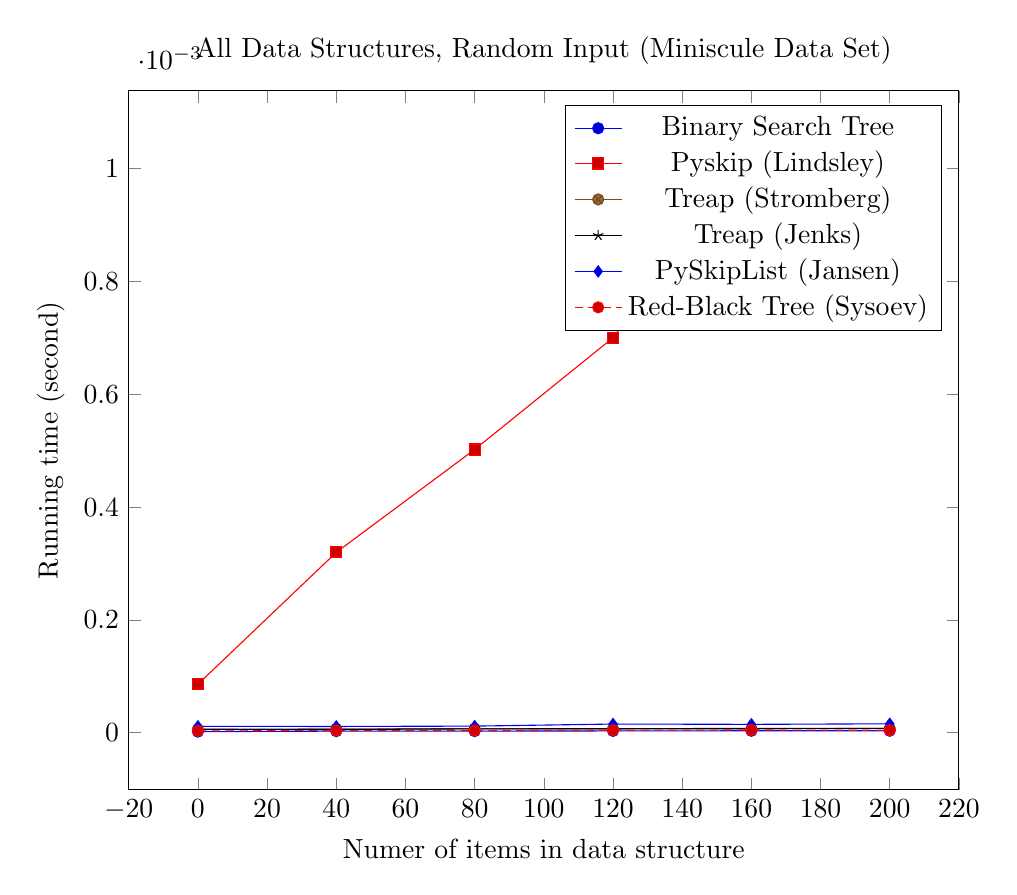
\begin{tikzpicture}
        \begin{axis}[
            xlabel={Numer of items in data structure},
            ylabel={Running time (second)},
            title={All Data Structures, Random Input (Miniscule Data Set)},
            width=\textwidth
        ]
		\addplot coordinates {
			(0, 1.987757222561044e-06)
			(40, 2.9214007664912305e-06)
			(80, 2.9214007664912335e-06)
			(120, 3.2828111705932418e-06)
			(160, 3.5538689736697333e-06)
			(200, 3.553868973669755e-06)
		};
		\addplot coordinates {
			(0, 8.601567617627793e-05)
			(40, 0.00031984820763027714)
			(80, 0.0005021496389660651)
			(120, 0.0007003531280823413)
			(160, 0.0010345673992756723)
			(200, 0.00090358624532237)
		};
		\addplot coordinates {
			(0, 5.812683999306678e-06)
			(40, 6.896915211612731e-06)
			(80, 7.228208082038501e-06)
			(120, 7.047502879989343e-06)
			(160, 7.047502879989343e-06)
			(200, 7.770323688194302e-06)
		};
		\addplot coordinates {
			(0, 6.294564538111835e-06)
			(40, 5.812683999306678e-06)
			(80, 6.957150278963376e-06)
			(120, 7.167973014690632e-06)
			(160, 7.710088620843657e-06)
			(200, 7.679971087168335e-06)
		};
		\addplot coordinates {
			(0, 1.1384427729213554e-05)
			(40, 1.1173604993486298e-05)
			(80, 1.180607320066529e-05)
			(120, 1.5480412309035185e-05)
			(160, 1.493829670288216e-05)
			(200, 1.5902057780489697e-05)
		};
		\addplot coordinates {
			(0, 3.28281117059348e-06)
			(40, 3.885161844097151e-06)
			(80, 3.855044310421829e-06)
			(120, 4.487512517600823e-06)
			(160, 4.9091579890525596e-06)
			(200, 4.427277450250178e-06)
		};
        \legend{Binary Search Tree, Pyskip (Lindsley), Treap (Stromberg), Treap (Jenks), PySkipList (Jansen), Red-Black Tree (Sysoev)}
        \end{axis}
    \end{tikzpicture}
    \caption{Average of 10 operations, benchmarked every 40, starting at 0.}
\end{figure}